%!TEX root = ../Chapter3.tex
\section{A Gamified Algorithm}\label{sec:lgc.game}

In this section, We present an asymptotically optimal algorithm for linear bandits BAI. Note that the present algorithm is asymptotically optimal for the general pure exploration game, which is however not the main focus of this thesis. Lecturers can refer to~\cite{degenne2020game} for more details.

Solely in this section, we make the following additional assumption that the set of parameter is bounded,
\begin{assumption}
\begin{leftbar}[assumptionbar]
    We assume that $\forall \btheta\in\Theta, \normm{\theta}\leq M$\,.
\end{leftbar}
\end{assumption}
This assumption is actually shared by most of the works on linear bandits (e.g. \citealt{abbasi-yadkori2011linear, soare2014linear}).

The bounded version of BAI is explicited in Section~\ref{sec:lgc.complexity.examples}. In particular we show how the boundedness of the parameter space affects the lower bound of Theorem~\ref{th:lb_genral}: The characteristic time $\Tstar(\theta)$ is reduced (or equivalently $\Tstar(\theta)^{-1}$ increases). This is not surprising since we add a new constraint in the optimization problem. This means that the algorithm should stop earlier. The counterpart of this improvement is that it is often difficult to compute the best response for nature. Indeed, for example, in BAI, there is an explicit expression of the best response, see Section~\ref{app:lgc.examples}. When the constraint $\normm{\lambda}\leq M$ is added there is no explicit expression anymore and one needs to solve an uni-dimensional optimization problem, see Lemma~\ref{lemma:lgc.lagrange_alternative}. To devise an asymptotically optimal algorithm without the boundedness assumption remains an open problem.


% , i.e for $i\in\cI$ and $w\in\interior{\Sigma_A}$ in the interior of the probability simplex of dimension $A-1$, find $\lambda^i$ such that
% \[
% \lambda^i \in \argmin_{\lambda\neg i}\normm{\theta - \lambda }_{V_{w}}\,.
% \]
% For example, in BAI, there is an explicit expression of the best response. Noting that, for $\astar\in\cA$, we have
% \[
% \min_{\lambda\neg \astar}\normm{\theta - \lambda }_{V_{w}} = \min_{a\neq \astar}\min_{\langle\lambda,a-\astar\rangle>0} \normm{\theta - \lambda }_{V_{w}}\,,
% \]
% the best response is then
% \begin{align}
% \lambda^{b} &= \theta - \frac{\max(\langle\theta,\astar-b \rangle,0) }{\normm{\astar-b}_{V_w^{-1}}^2} V_w^{-1}(\astar - b) \label{eq:best_response_bai}
% \\
% \text{for }b&\in\argmin_{a\neq \astar}\normm{\theta - \lambda^{a} }_{V_{w}}\nonumber.
% \end{align}
% When the constraint $\normm{\lambda}\leq M$ is added there is no explicit expression anymore and one needs to solve an uni-dimensional optimization problem, see Lemma~\ref{lemma:lgc.lagrange_alternative}.


%Note that in the proof of Theorem~\ref{thm:sample_complexity} we only use two times the boundedness assumption, first in the definition of the threshold $\beta(t,\delta)$ (see Theorem~\ref{th:confidence_beta}) to handle the bias induced by the regularization. Second, since the regret of AdaHedge is proportional to the maximum of the upper confidence bounds $U_s^{i,a}$, we need to ensure that they are bounded.

% And there exists pathological pure exploration problems where even the quantity uppper bounded by $U_s^{i,a}$, namely $\normm{\theta-\lambda}_{aa^\top}^2$ where $\lambda\in\argmin_{\lambda'\in\neg i}\normm{\theta -\lambda}$ is unbounded\todo{I don't understand what this means.}. See for example Appendix~G.3 by \citet{menard2019lma}.


In this chapter, we study the problem from a \emph{zero-sum game} point of view inspired by~\cite{degenne2019pure}. We describe \LG{}, detailed in Algorithm~\ref{alg:lgc}. The full analysis of the algorithm is omitted as well as a convexified version \LGC{} -- also asymptotically optimal itself -- as they are not the main focus of this thesis. Lecturers can refer to~\cite{degenne2020game} for the complete proofs.

\subsection{Notations}
\paragraph{Counts.} At each round $t$ the algorithms will play an arm $a_t$ and choose (fictitiously) an answer $i_t$. We denote by $N_t^{a,i} \eqdef\sum_{s=1}^t \ind_{\{(a_t,i_t)=(a,i)\}}$ the number of times the pair $(a,i)$ is chosen up to and including time $t$, and by $N_t^a =\sum_{i\in\cI} N_s^{a,i}$ and $N_t^i =\sum_{a\in\cI} N_s^{a,i}$ the partial sums. The vectors of counts at time $t$ is denoted by $N_t \eqdef (N_t^a)_{a\in\cA}$
and when it is clear from the context we will also denote by $N_t^a = (N_t^{a,i})_{i\in\cI}$ and $N_t^i = (N_t^{a,i})_{i\in\cI}$ the vectors of partial counts.

\paragraph{Regularized least square estimator.} We fix a regularization parameter $\eta > 0$. The regularized least square estimator for the parameter $\theta\in \mathcal M$ at time $t$ is
\[
\htheta_{t} = (V_{N_t} + \eta I_d)^{-1} \sum_{s=1}^t Y_s a_s\,,
\]
where $I_d$ is the identity matrix. By convention $\htheta_0 = 0$.


\subsection{The \LG{} algorithm}

\begin{algorithm}[ht]
\centering
\caption{\LG}
\label{alg:lg}
\begin{algorithmic}[1]
    \State {\bfseries Input:} Agent learners for each answers $(\cL^i_w)_{i\in\cI}$, threshold $\beta(\cdot,\delta)$
    \For{t = 1 \ldots}
        \State \textit{// Stopping rule}
        \If{{$\max_{i\in\cI}\inf_{\lambda\in\neg i} \frac{1}{2}\normm{\htheta_{t-1}-\lambda}^2_{V_{N_{t-1}}}\geq\! \beta(t-1,\delta)$}}
            \State \texttt{stop} 
            \State {\bfseries Return} $\hi = \istar(\hat{\theta}_{t-1})$
        \EndIf
        \State \textit{// Best answer}
        \State $i_{t} = \istar(\hat{\theta}_{t-1})$
        \State \textit{// Agent plays first}
        \State \texttt{get} $w_{t}$ \texttt{from} $\cL^{i_t}_w$
        \State \texttt{update} $W_{t}=W_{t-1}+w_{t}$
        \State \textit{// Best response for the nature}
        \State $\lambda_{t} \in \argmin_{\lambda\in\neg i_t}\normm{\htheta_{t-1}-\lambda}^2_{V_{w_{t}}}$
        \State \textit{// Feed optimistic gains}
        \State \texttt{feed learner} $\cL_w^{i_{t}}$ \texttt{with} $g_{t}(w) = \sum_{a\in\cA}w^a U_t^a/2$
        \State \textit{// Track the weights}
        \State \texttt{pull} $a_{t}\in \argmin_{a\in \mathcal A } N_{t-1}^{a} - W_{t}^{a}$
   \EndFor
\end{algorithmic}
\end{algorithm}

% \begin{algorithm}[tb]
% \centering
% \caption{\LGC}
% \label{alg:lgc}
% \begin{algorithmic}[1]
%     \State {\bfseries Input:} Agent learner $\cL_{\tw}$, threshold $\beta(\cdot,\delta)$
%     \For{t = 1 \ldots}
%         \State \textit{// Stopping rule}
%         \If{ {\small $\max_{i\in \cI} \inf_{\lambda\in\neg i} \frac{1}{2}\normm{\htheta_{t-1}-\lambda}^2_{V_{N_{t-1}}}\geq \beta(t-1,\delta)$}}
%             \State {\bfseries stop} and {\bfseries return} $\hi = \istar(\hat{\theta}_{t-1})$. 
%         \EndIf
%         \State \textit{// Agent plays first}
%         \State \texttt{get} $\tw_{t}$ \texttt{from} $\cL_{\tw}$ 
%         \State \texttt{update} $\tW_{t}=\tW_{t-1}+\tw_{t}$
%         \State \textit{// Best response for the nature}
%         \State $\forall i\in\cI$, $\tlambda^i_{t} \in \argmin_{\lambda\in\neg i}\normm{\htheta_{t-1}-\lambda}^2_{V_{\tw^i_{t}}}$
%         \State \textit{// Feed optimistic gains}
%         \State \texttt{feed learner} $\cL_{\tw}$ \texttt{with} {$g_{t}(\tw) =\sum_{(a,i)\in\cA\times\cI} \tw^{a,i} U_t^{a,i}/2$}
%         \State \textit{// Track the weights}
%         \State \texttt{pull} $(a_{t},i_{t})\in \argmin_{(a,i)\in \mathcal A \times \mathcal I} N_{t-1}^{a,i} - \tW_{t}^{a,i}$
%     \EndFor
% \end{algorithmic}
% \end{algorithm}

\paragraph{Stopping rule and decision rules.}
Our algorithms share the same stopping rule. Following \citet{garivier2016tracknstop}, our algorithms stop if a generalized likelihood ratio exceeds a threshold. It stops if
\begin{align}
\label{eq:def_chernoff_stopping}
\max_{i\in \mathcal I} \inf_{\lambda_i \in \neg i}\frac{1}{2}\Vert \tilde{\theta}_t - \lambda_i \Vert^2_{V_{N_t}}
> \beta(t,\delta)\,,
\end{align}
and return {\small $\displaystyle \istar_t\! \in\! \argmax_{i\in \mathcal I}\! \inf_{\lambda_i \in \neg i}\Vert \tilde{\theta}_t - \lambda_i \Vert^2_{V_{N_t}}/2$}.


These stopping and decision rules ensure that the \LG{} is $\delta$-correct regardless of the sampling rule used, see lemma below\footnote{The fact that $\tau_\delta <+\infty$ is a consequence of our analysis, see Appendix~\ref{app:lgc.proof}.} proved in Appendix~\ref{app:lgc.lemmas}.

\begin{lemma}
\label{lem:chernoff_stopping rule_pac}
Regardless of the sampling rule, the stopping rule~\eqref{eq:def_chernoff_stopping} with the threshold
{\small\begin{equation} \label{eq:def_beta}
\beta(t,\delta) =\left( \sqrt{\log\!\left( \frac{1}{\delta}\right)+\frac{d}{2}\log\!\left(1+\frac{t L^2}{\eta d} \right)} +\sqrt{\frac{\eta}{2}}M\right)^2\!\!\!,
\end{equation}}
satisfy $ \P_{\theta}\big(\tau_{\delta} < \infty \wedge \istar_t \neq \istar(\theta)\big) \leq \delta$.
\end{lemma}
% This stopping and decision rules ensures that the algorithm is $\delta$-correct regardless of the sampling rule used (see \citealt{garivier2016tracknstop} for a proof), hence the following theorem is immediate.
% \begin{theorem}
% Algorithms~\ref{alg:lg} and~\ref{alg:lgc} are $\delta$-correct.
% \end{theorem}
Our contribution is a sampling rule that minimizes the sample complexity when combined with these stopping and decision rules.
We now explain our sampling strategy to ensure that the stopping threshold is reached as soon as possible.

\paragraph{Saddle point computation.}
Suppose in this paragraph, for simplicity, that the parameter vector $\theta$ is known. By the definition of the stopping rule and the generalized likelihood ratio, as long as the algorithm does not stop,
\begin{align*}
\beta(t,\delta)
&\ge \inf_{\lambda\in \neg i^\star(\theta)} \sum_{a\in \cA} N_t^a \Vert \theta - \lambda \Vert^2_{a a^\top}/2 \: .
\end{align*}
If we manage to have $N_t \approx t w^\star(\theta)$ (the optimal pulling proportions at $\theta$), then this leads to $\beta(t,\delta) \ge t T^\star(\theta)^{-1}$ and, solving that equation, we have asymptotic optimality.

Since there is only one correct answer, the parameter $\theta$ belongs to all sets $\neg i$ for $i\neq \istar(\theta)$. Hence
\begin{align*}
&\inf_{\lambda\in \neg i^\star(\theta)}\frac{1}{2} \sum_{a\in \cA} N_t^a \Vert \theta - \lambda \Vert^2_{a a^\top}
\\&\geq \inf_{\tlambda_t\in \prod_i (\neg i)}\frac{1}{2}\sum_{(a,i)\in \cA\times\cI}\!\!\!\!\! N_t^{a,i} \Vert \theta - \tlambda^i \Vert^2_{a a^\top}.
\end{align*} Introducing the sum removes the dependence in the unknown $i^*(\theta)$. \LGC then uses an agent playing weights w in $\Sigma_{\cA\cI}$. \LG does not use that sum over answers, but uses a guess for $\istar(\theta)$. Its analysis involves proving that the guess is wrong only finitely many times in expectation.

Our sampling rule implements the lower bound game between an agent, playing at each stage $s$ a weight vector $\tw_s$ in the probability simplex $\Sigma_{A\times I}$, and nature, who computes at each stage a point $\lambda_s^i \in \neg i$ for all $i\in \mathcal I$. We additionally ensure that $N_t^{a,i} \approx \sum_{s=1}^t \tw_s^{a,i}$. Suppose that the sampling rule is such that at stage $t$, a $\varepsilon_t$-approximate saddle point is reached for the lower bound game, see Lemma~\ref{lem:sion_convexify}. That is,
\begin{align*}
&\inf_{\tlambda \in \prod_{i}(\neg i)} \sum_{s=1}^t \sum_{(a,i)\in \cA\times\cI} \tw_s^{i,a} \Vert \theta - \tlambda^i \Vert^2_{a a^\top}/2 +\varepsilon_t
\\
&\ge \sum_{s=1}^t \sum_{(a,i)\in \cA\times\cI} \tw_s^{i,a} \Vert \theta - \tlambda_s^i \Vert^2_{a a^\top}/2
\\
&\ge\max_{(a,i)\in \cA\times\cI} \sum_{s=1}^t \Vert \theta - \tlambda_s^i \Vert^2_{a a^\top}/2 - \varepsilon_t \: .
\end{align*}
Then if the algorithm did not stop, it verifies, using Lemma~\ref{lem:sion_convexify},
\begin{align*}
\beta(t,\delta)
&\ge t \max_{(a,i)\in \cA\times\cI} \frac{1}{t}\sum_{s=1}^t \Vert \theta - \tlambda_s^i \Vert^2_{a a^\top}/2 - 2\varepsilon_t
\\
&\ge t \inf_{\tq \in \mathcal \prod_{i\in \mathcal I}\cP(\neg i)} \! \max_{(a,i)\in \cA\times\cI} \!\!\!\! \mathbb{E}_{\lambda^i\sim q^i}\Vert \theta \! - \! \tlambda^i \Vert^2_{a a^\top}/2 \! - \! 2\varepsilon_t\\
&= t T^\star(\theta)^{-1} - 2 \varepsilon_t \: .
\end{align*}
Solving that equation, we get asymptotically the wanted $t\lesssim T^\star(\theta) \log(1/\delta)$.

We implement the saddle point algorithm by using AdaHedge for the agent (a regret minimizing algorithm of the exponential weights family), and using best-response for the nature, which plays after the agent. Precisely \LG uses $|\cI|$ learners $\cL_w^i$, one for each possible guess of $\Istar(\btheta)$ with the gains. For $i\in\cI$, the learner $\cL_w^i$ is also AdaHedge but only on $\Sigma_K$ with the gains (when the guess is $i$)
\[
    g_t^\theta(w) = \frac{1}{2} \sum_{a\in\cA}  w^{a} \Vert \theta - \lambda_s^i \Vert^2_{a a^\top}\,.
\]
$\varepsilon_t$ is then the sum of the regrets of the two players. Best-response has regret 0, while the regret of AdaHedge is $O(\sqrt{t})$ for bounded gains, as seen in the following lemma, taken from \citet{derooij2014hedge}.
%\todo{define the learners $\cL_w^i$ here}
\begin{lemma}\label{lem:adahedge}
On the online learning problem with $K$ arms and gains $g_s(w) = \sum_{k\in[K]} w^k  U_s^k$ for $s\in[t]$, AdaHedge, predicting $(w_s)_{s\in[t]}$, has regret
\begin{align*}
%R_T &\le 2\sqrt{(\sigma L_T - \frac{L_T^2}{T})\log(K)} + \sigma(2+\log(K)16/3) \: ,\\
R_t&:= \max_{w\in\Sigma_K}\sum_{s=1}^t g_s(w) -g_s(w_s) \\
&\le 2\sigma\sqrt{t\log(K)} + 16\sigma(2+\log(K)/3) \: ,\\
\text{where }
\sigma &= \max_{s\le t}  (\max_{k\in[K]}U_s^{k}- \min_{k\in[K]}U_s^{k}) \:.\\
%L_T &= \sum_{t=1}^T (\max_{k\in[K]}U_t^{k} - U_t^{\star}) \le T \sigma \: .
\end{align*}
\end{lemma}
Other combinations of algorithms are possible, as long as the sum of their regrets is sufficiently small. At each stage $t\in\NN$, both algorithms advance only by one iteration and as time progresses, the quality of the saddle point approximation improves. This is in contrast with \Track \cite{garivier2016tracknstop}, in which an exact saddle point is computed at each stage, at a potentially much greater computational cost.

\paragraph{Optimism.} The above saddle point argument would be correct for a known game, while our algorithm is confronted to a game depending on the unknown parameter $\theta$. Following a long tradition of stochastic bandit algorithms, we use the principle of Optimism in Face of Uncertainty. Given an estimate $\hat{\theta}_{t-1}$, we compute upper bounds for the gain of the agent at $\theta$, and feed these optimistic gains to the learner. Precisely, given the best response $\lambda_t^i \in \neg i$ we define,
\begin{align*}
U_t^{a,i} =\left\{
\begin{array}{ll}
\max_{\xi} \quad & \min\big(\Vert \xi - \lambda_t^i \Vert^2_{a a^\top},4L^2M^2\big)\\
\text{s.t.}\quad & \Vert \hat{\theta}_{t-1} - \xi \Vert^2_{V_{N_{t-1}}+\eta I_d} \le 2h(t)
\end{array}
\right. \: ,
\end{align*}
where $h(t)=\beta(t, 1/t^3)$ is some exploration function. We clipped the values, using that $\cM$ and $\cA$ are bounded to ensure bounded gains for the learners. Under the event that the true parameter verifies $\Vert \hat{\theta}_{t-1} - \theta \Vert^2 \le 2 h(t)$, this is indeed an optimistic estimate of $\Vert \theta - \lambda_t^i \Vert^2_{a a^\top}$. Note that $U_t^{a,i}$ has a closed form expression, see Appendix~\ref{app:lgc.proof}. The optimistic gain is then, for \LGC (see Algorithm~\ref{alg:lg} for the one of \LG),
\[
g_t(\tw) = \frac{1}{2} \sum_{(a,i)\in\cA\times\cI}  \tw^{a,i} U_t^{a,i}\,.
\]


\paragraph{Tracking.} In both Algorithm~\ref{alg:lg} and~\ref{alg:lgc}, the agent plays weight vectors in a simplex. Since the bandit procedure allows only to pull one arm at each stage, our algorithm needs a procedure to transcribe weights into pulls. This is what we call tracking, following \citet{garivier2016tracknstop}. The choice of arm (or arm and answer) is
\begin{align*}
a_{t+1}          &\in \argmin_{a\in \mathcal A } N_{t}^{a} - W_{t+1}^{a} & \text{ for Algorithm~\ref{alg:lg},}\\
(a_{t+1},i_{t+1})&\in \argmin_{(a,i)\in \mathcal A \times \mathcal I } N_{t}^{a,i} - \tW_{t+1}^{a,i} & \text{ for Algorithm~\ref{alg:lgc}.}
\end{align*}
This procedure guarantees that for all $t\in\NN, u \in \mathcal U$, with $\mathcal U = \mathcal A$ (resp. $\mathcal U =\cI\times\cA$) for Algo.~\ref{alg:lg} (resp. Algo.~\ref{alg:lgc}), $- \log (|\mathcal U|) \le N_t^{u} - W_t^{u} \le 1$. That result is due to~\citet{degenne2020structure}.

\begin{theorem}\label{thm:sample_complexity}
For a regularization parameter\footnote{This condition is a simple technical trick to simplify the analysis. An $\eta$ independent of $A$,$L$,$M$ will lead to the same results up to minor adaptations of the proof.} $\eta \geq 2(1+\log(A))AL^2+M^2$, for the threshold $\beta(t,\delta)$ given by~\eqref{eq:def_beta}, for an exploration function $h(t)=\beta(t,1/t^3)$, \LG and \LGC are $\delta$-correct and asymptotically optimal. That is, they verify for all $\theta\in \cM$,
\begin{align*}
\limsup_{\delta\to 0}\frac{\mathbb{E}_\theta[\tau_\delta]}{ \log 1/\delta} \le \Tstar(\theta) \: .
\end{align*}
\end{theorem}
The main ideas used in the proof are explained above. The full proof is in Appendix~\ref{app:lgc.proof} with finite $\delta$ upper bounds.

\subsection{Experiments}\label{sec:lgc.game.experiments}

In this section, we provide technical details of our experiments. We also share a few insights over different aspects of implementations of different pure exploration linear bandits algorithms. In particular, we propose a new Frank-Wolfe-typed heuristic to solve generic $\cA\cB$-design.

Besides our algorithms, we implement the following algorithms, all using the same stopping rule (more discussion given in Appendix~\ref{app:lgc.stopping}): uniform sampling, the greedy version of \XYS (including $\gopt$-allocation and $\xyopt$-allocation), \XYA, and the greedy version of \LGapE. We skip \GLUCB/\GLGapE since they are more or less equivalent to \LGapE in the scope of this paper.

\paragraph{Implementation details.}
We give more clarifications on each individual algorithm implemented.

\begin{itemize}
	\item For our algorithms \LG and \LGC, we implemented the version with the boundedness assumption.
	\item For \LGapE We implemented the greedy version, that is, pull the arm 
	\[
	    \argmin_{a\in\cA} \normm{a_{i_t}-a_{j_t}}_{(V_{N_t}+aa^\top)^{-1}}^2
	\]
	with $i_t = i^\star(\hat\theta_t)$ and $j_t = \argmax_{j\neq i_t}\langle\hat\theta_t,a_{j}-a^\star(\hat\theta_t)\rangle + \normm{a^\star(\hat\theta_t) - a_{j_t}}_{V_{N_t}^{-1}} \sqrt{2\beta(t,\delta)}$. Note that this version does not have a theoretical guarantee in the general case. However, as we stated in Section~\ref{sec:lgc.related_work}, the \GLUCB proposed by~\citet{zaki2019maxoverlap} is equivalent to this greedy version of \LGapE, and they provided an analysis for the 2-arm and 3-arm case. \LGapE is designed for $\epsilon$-best-arm identification, we set $\epsilon=0$ in our experiments to make sure that it outputs the optimal one.
	\item For \XYS, we implemented the greedy incremental version for both $\gopt$-allocation and $\xyopt$-allocation, that allows us to avoid the optimal design-computing step. To implement the non-greedy version, readers are invited to look at next Section~\ref{sec:lgc.experiments.complexity} where we discuss in detail the computation of $\cA\cB$-optimal design.
	\item For \XYA, it requires a hyper-parameter that characterizes the length of each phase. We set that hyper-parameter to $0.1$ as done by~\citet{soare2014linear}.
\end{itemize}

% \paragraph{Technical details.} All the algorithms and experiments are implemented in \lstinline{Julia 1.3.1}, and plots are generated using the \lstinline{StatsPlots.jl} package. Other external dependencies are: \lstinline{JLD2.jl, Distributed.jl, IterTools.jl, CPUTime.jl, LaTeXStrings.jl}.

% \paragraph{For reproducibility.} To rerun our code, your need to have Julia installed, then unzip \lstinline{code.zip} and do the following in your terminal.

% \begin{lstlisting}
%   $ cd PATH/TO/THE/FOLDER/code/linear
%   $ julia
%   julia> include("experiment_bai1.jl") # reproduce Fig.1
%   julia> include("viz_bai1.jl") # visualization
%   julia> include("experiment_bai2.jl") # reproduce Fig.2
%   julia> include("viz_bai2.jl") # visualization
% \end{lstlisting}

%\subsubsection{Arm generation.} In Section~\ref{sec:experiments}, we need to generate arms uniformlly from a unit sphere of arbitrary dimension. This can be done using Algorithm~\ref{alg:generation}, it can be trivially extended to higher dimension.
%
%\begin{algorithm}[ht]
%   \caption{Generating arms from the 2D unit sphere (Box-Mueller)}
%   \label{alg:generation}
%\begin{algorithmic}
%        \State $u \sim \cN(0,1)$
%        \State $v \sim \cN(0,1)$
%        \State $(x, y) = (u, v)/\normm{(x, y)}_2$
%        \RETURN $x, y$
%\end{algorithmic}
%\end{algorithm}

\paragraph{Implementation trick.}
Matrix inversion is a costly step that should be avoided at best. For linear bandits, in particular, we need to inverse the (regularized) design matrix $\bB^{\lambda}_n$, which is renewed with a rank-1 update at each time step. Applying Sherman-Morrison formula allows us thus to only update its inverse incrementally, that releases a huge burden of computation.

Indeed, beginning with $\bB^{\lambda}_0 \eqdef \lambda\1_d$, we have
\[
    \forall t\geq 0, \quad \bB^{\lambda}_{t+1} = \bB^{\lambda}_t + \hat{\bx}_{t+1}\hat{\bx}_{t+1}\transpose,
\]
thus using Sherman-Morrison formula we have
\[
    \forall t\geq 0, \quad (\bB^{\lambda}_{t+1})^{-1} = (\bB^{\lambda}_t)^{-1} - \frac{(\bB^{\lambda}_t)^{-1}\hat{\bx}_{t+1}\hat{\bx}_{t+1}\transpose(\bB^{\lambda}_t)^{-1}}{1+\normm{\hat{\bx}_{t+1}}_{(\bB^{\lambda}_t)^{-1}}^2}.
\]

The posterior mean vector and covariance matrix can then be easily expressed in terms of $(\bB^{\lambda}_t)^{-1}$. Let $\bz_t \eqdef \sum_{s=1}^t y_s\hat{\bx}_s$, we obtain
\[
    \hat{\btheta}_n^{\lambda} = (\bB^{\lambda}_t)^{-1}\bz_t \quad \text{and} \quad \hat{\bSigma}_n = \sigma^2 (\bB^{\lambda}_t)^{-1}\,.
\]

\paragraph{Experimental setting.}

Usual sampling rules for classical BAI may not work for the linear case. This can be understood on a well-studied instance already discussed by~\citet{soare2014linear,xu2018linear}, which encapsulates the difficulty of BAI in a linear bandit, and thus is the first instance on which we test our algorithms. In this instance, arms are the canonical basis  $a_1 = e_1, a_2 = e_2, a_d = e_d$, plus an additional disturbing arm $a_{d+1} = (\cos(\alpha), \sin(\alpha), 0, \ldots, 0)^\top$, and a true regression parameter $\theta$ equal to $e_1$. In this problem, the best arm is always $a_1$, but when the angle $\alpha$ is small, the disturbing arm $a_{d+1}$ is hard to discriminate from $a_1$. As already argued by~\citet{soare2014linear}, an efficient sampling rule for this problem instance would rather pull $a_2$ in order to reduce the uncertainty in the direction $a_1-a_{d+1}$. Naive adaptation of classical BAI algorithms cannot deal with that situation naturally. We further use a simple set of experiments to justify that intuition. We run our two algorithms and the one of~\citet{degenne2019game} that we call \texttt{DKM} over the problem instance whence $d=2$, $\delta=0.01$ and $\alpha=0.1$. We show the number of pulls for each arm averaged over 100 replications of experiments in Table~\ref{table:pulls}. We see that, indeed, \texttt{DKM} pulls too much $a_3$, while our algorithms focus mostly on $a_2$.

\begin{table}[t!]\centering
%\def\arraystretch{1.2}
\begin{tabular}{|c|c|c|c|}
 \hline
 & \LG & \LGC & \texttt{DKM} \\
 \hline
 \textbf{$a_1$} & $1912$ & $1959$ & $1943$ \\
 \hline
 \textbf{$a_2$} & $5119$ & $4818$ & $4987$ \\
 \hline
 \textbf{$a_3$} & $104$ & $77$ & $1775$ \\
 \hline
 \textbf{Total} & $7135$ & $\bf{6854}$ & $8705$ \\
 \hline
\end{tabular}
\caption{Average number of pulls of \LG and \LGC (against \texttt{DKM}) for each arm.}
\label{table:pulls}
\end{table}

\paragraph{Experimental results}

We benchmark our two sampling rules against others from the literature. %Note that the main purpose of this paper is to propose algorithms with asymptotic optimality while being practically usable, but we do not claim to have the best performing ones.
We test over two synthetic problem instances, with the first being the previous counter-example. We set $d=2$, $\alpha=\pi/6$. Fig.~\ref{fig:sample_complexity_1} shows the empirical stopping time of each algorithms averaged over 100 runs, with a confidence level $\delta=0.1, 0.01, 0.0001$ from left to right. Our two algorithms show competitive performance (the two leftmost boxes on each plot), and are only slightly worse than \LGapE.

\begin{figure}[ht]
 \centering
 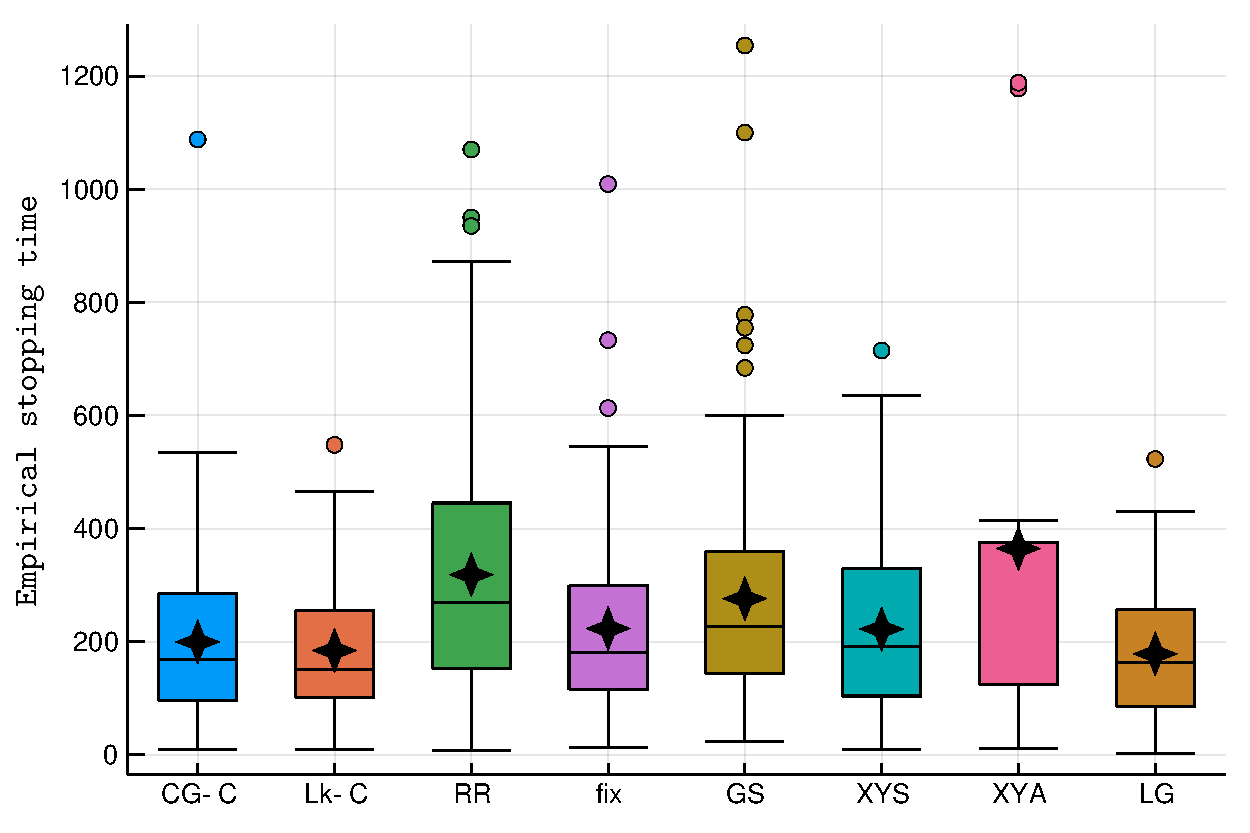
\includegraphics[clip, width= 0.33\textwidth]{Chapter4/img/bai_sin_0-1}
 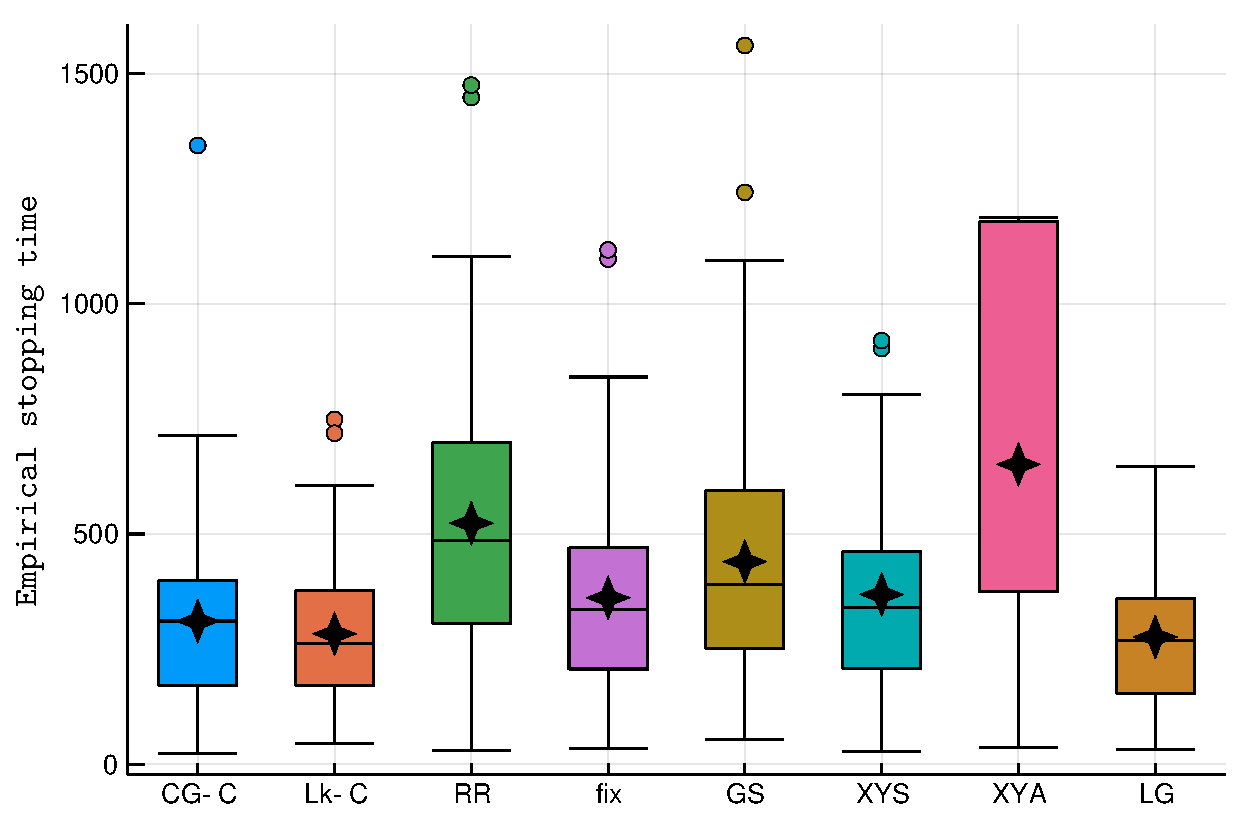
\includegraphics[clip, width= 0.33\textwidth]{Chapter4/img/bai_sin_0-01}
 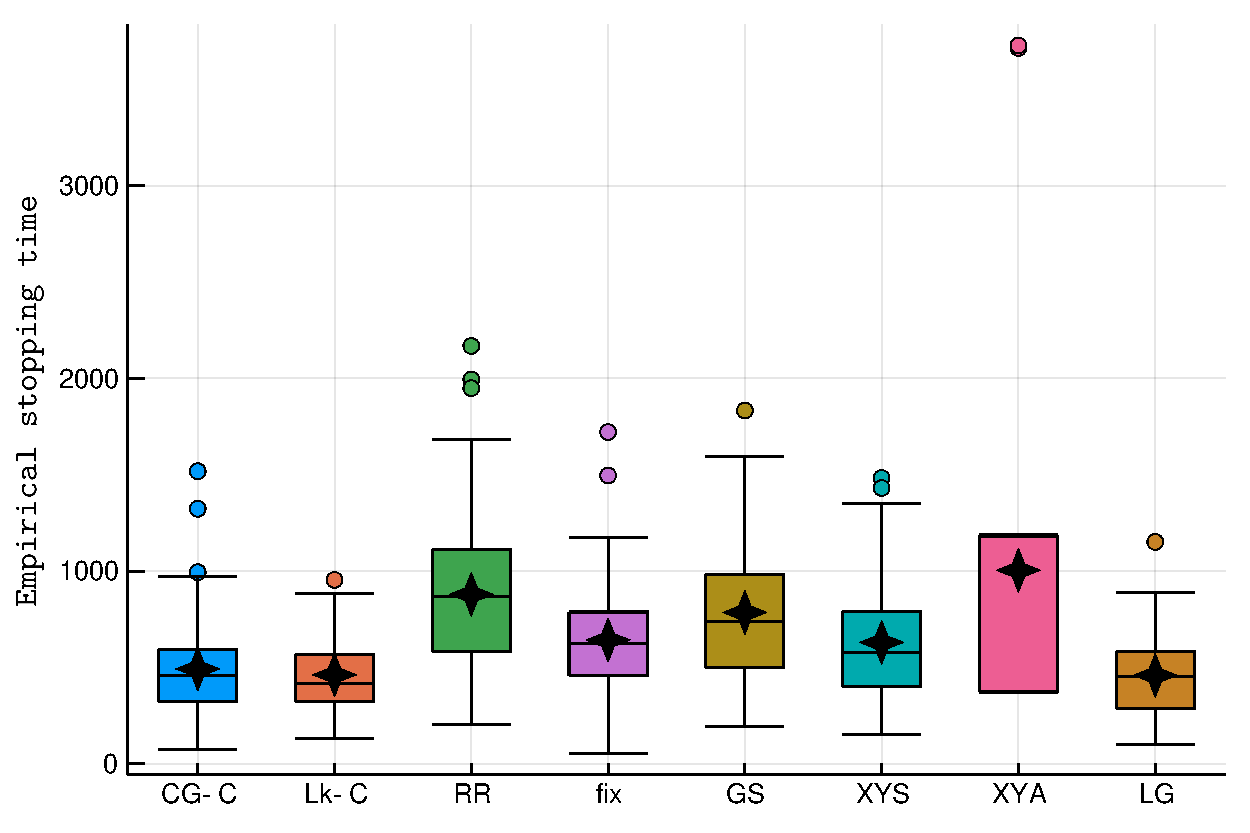
\includegraphics[clip, width= 0.33\textwidth]{Chapter4/img/bai_sin_0-0001}
 \caption{Sample complexity of different linear BAI sampling rules over the usual counter-example with $\delta=0.1, 0.01, 0.0001$ respectively. CG = \LGC,  Lk = \LG, RR = uniform sampling, fix = tracking the fixed weights, GS = \XYS with $\gopt$-allocation, XYS = \XYS with $\xyopt$-allocation, LG = \LGapE. The mean stopping time is represented by a black cross.}
 \label{fig:sample_complexity_1}
\end{figure}

For the second instance, we consider 20 arms randomly generated from the unit sphere $\mathbb{S}^{d-1}\eqdef\{a\in\R^d; \normm{a}_2=1\}$. We choose the two closest arms $a, a'$ and we set $\theta = a + 0.01(a'-a)$ so that a is the best arm. This setting has already been considered by~\citet{tao2018alba}. We report the same box plots over 100 replications as before with increasing dimension in Fig.~\ref{fig:sample_complexity_2}. More precisely, we set $d=6, 8, 10, 12$ respectively, and always keep a same $\delta = 0.01$. Our algorithms consistently show strong performances compared to other algorithms apart from \LGapE. Moreover, we can see that in these random examples, \LGC works better than the non-confexified one, and is even competitive compared to \LGapE.


\begin{figure}[ht]
 \centering
 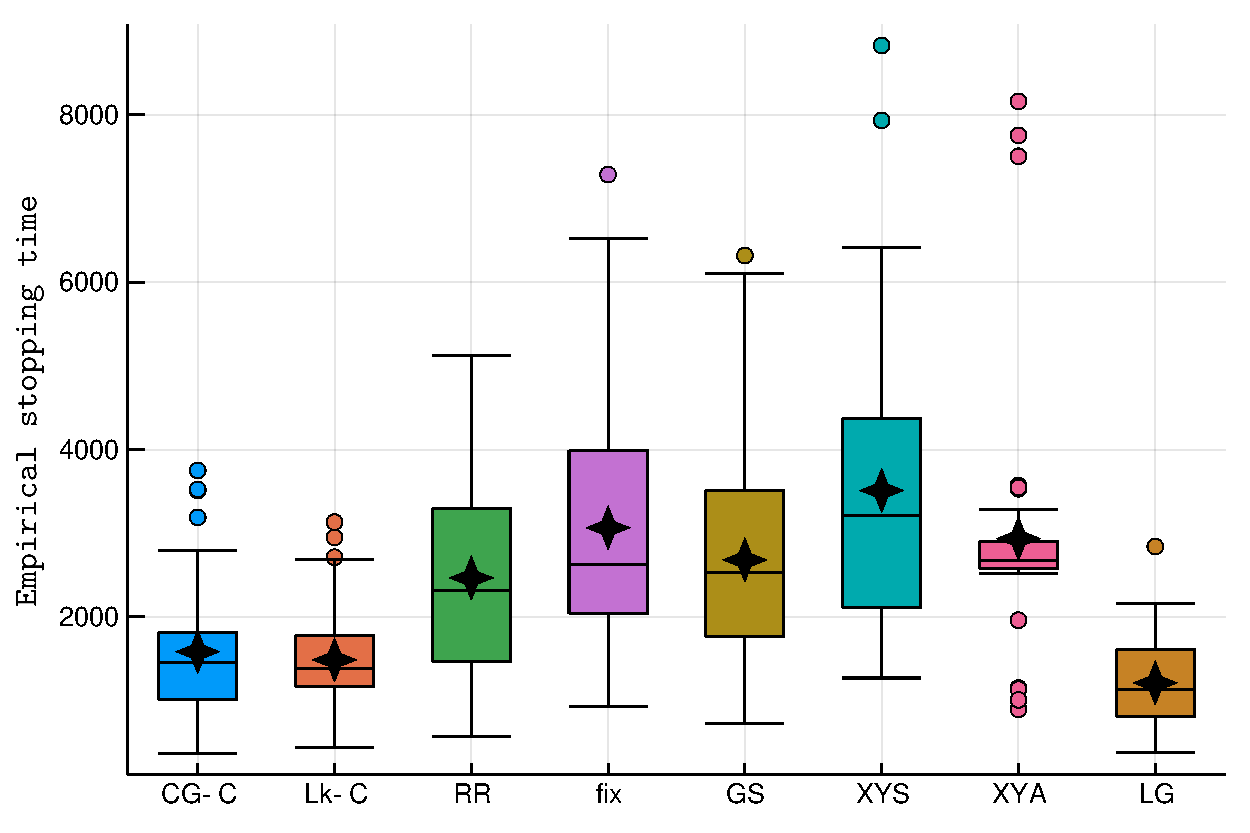
\includegraphics[clip, width= 0.33\textwidth]{Chapter4/img/bai_dim_6}
 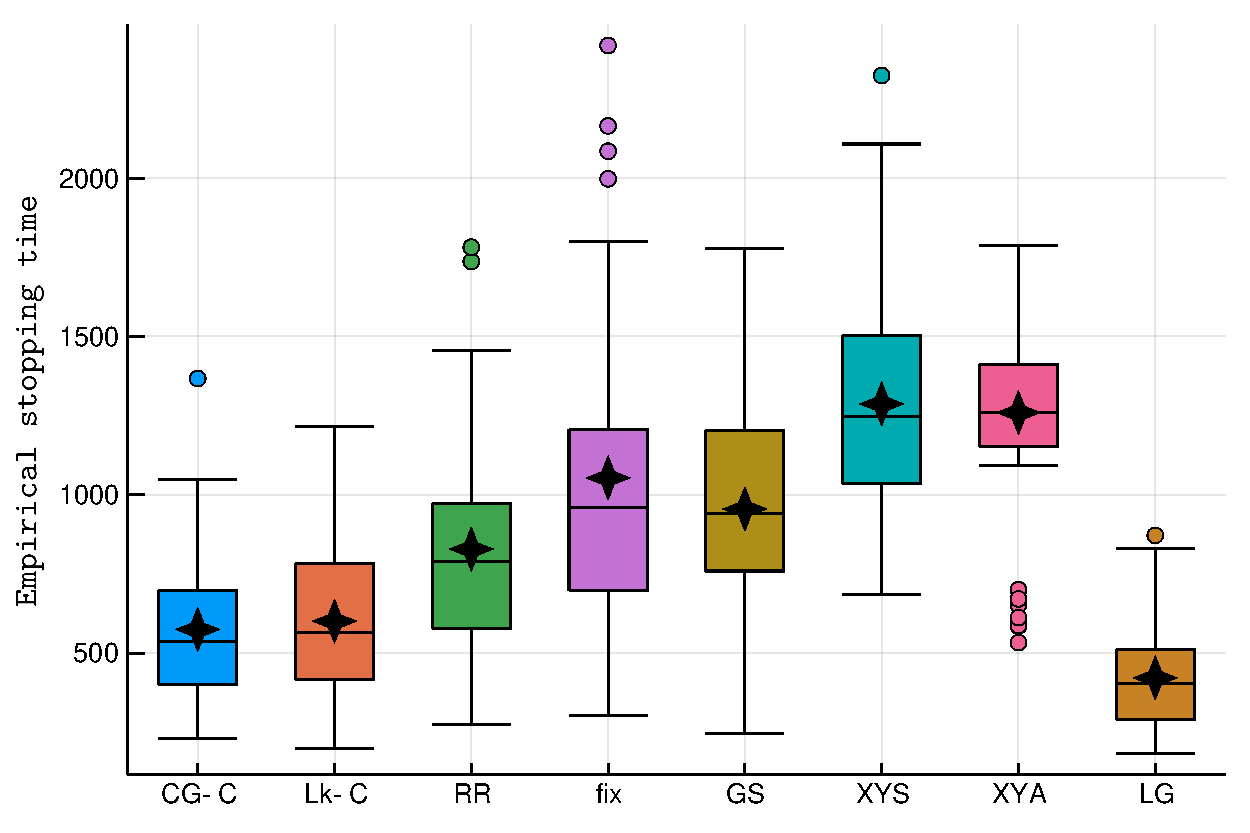
\includegraphics[clip, width= 0.33\textwidth]{Chapter4/img/bai_dim_8}
 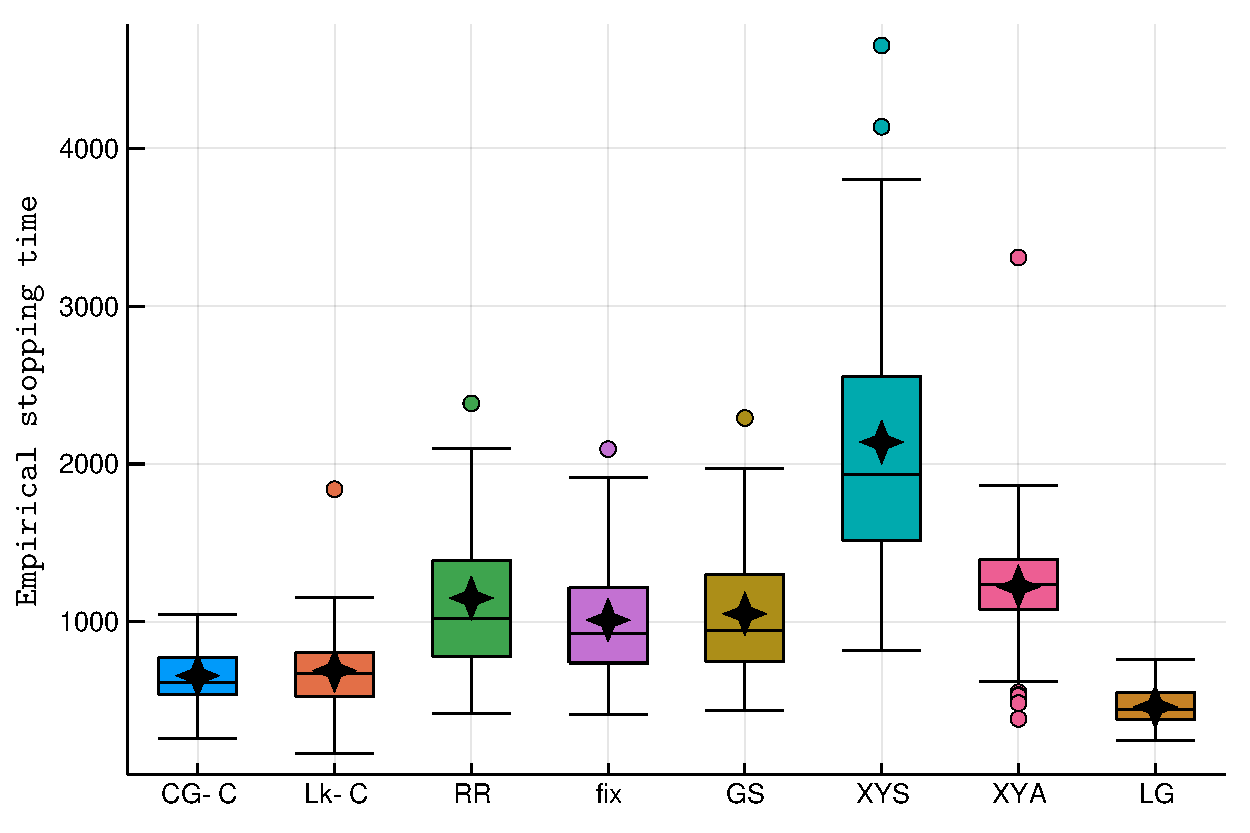
\includegraphics[clip, width= 0.33\textwidth]{Chapter4/img/bai_dim_10}
 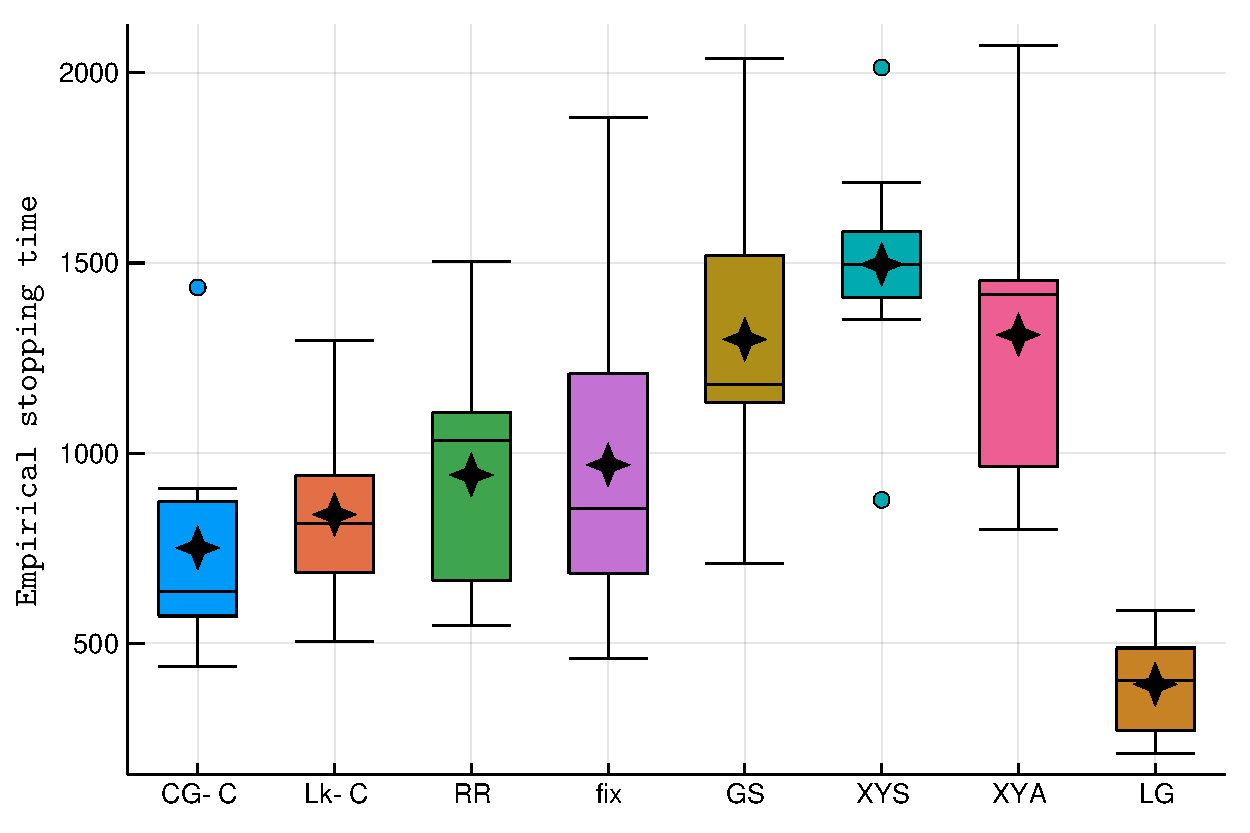
\includegraphics[clip, width= 0.34\textwidth]{Chapter4/img/bai_dim_12}
 \caption{Sample complexity of different linear BAI sampling rules over random unit sphere vectors with $d=6, 8, 10, 12$ from left to right.}
 \label{fig:sample_complexity_2}
\end{figure}

We stress that although the main focus of this chapter is theoretical, with algorithms that are asymptotically optimal, our methods are also competitive with earlier algorithms experimentally.

